%%%%%%%%%%%%%%%%%%%%%%%%%%%%%%%%%%%%%%%%%
% Beamer Presentation
% LaTeX Template
% Version 1.0 (10/11/12)
%
% This template has been downloaded from:
% http://www.LaTeXTemplates.com
%
% License:
% CC BY-NC-SA 3.0 (http://creativecommons.org/licenses/by-nc-sa/3.0/)
%
%%%%%%%%%%%%%%%%%%%%%%%%%%%%%%%%%%%%%%%%%

%----------------------------------------------------------------------------------------
%	PACKAGES AND THEMES
%----------------------------------------------------------------------------------------

\documentclass[usenames,dvipsnames]{beamer}

\mode<presentation> {

% The Beamer class comes with a number of default slide themes
% which change the colors and layouts of slides. Below this is a list
% of all the themes, uncomment each in turn to see what they look like.



\usepackage{amsmath}
\usepackage[customcolors,shade]{hf-tikz}
\usepackage{blindtext}
\usepackage{pst-node,graphicx}
\usepackage[hoptionsi]{reflectgraphics}


%\usetheme{default}
%\usetheme{AnnArbor}
%\usetheme{Antibes}
%\usetheme{Bergen}
%\usetheme{Berkeley}
%\usetheme{Berlin}
%\usetheme{Boadilla}
%\usetheme{CambridgeUS}
%\usetheme{Copenhagen}
%\usetheme{Darmstadt}
%\usetheme{Dresden}
%\usetheme{Frankfurt}
%\usetheme{Goettingen}
%\usetheme{Hannover}
%\usetheme{Ilmenau}
%\usetheme{JuanLesPins}
%\usetheme{Luebeck}
\usetheme{metropolis}
%\usecolortheme{crane}
%\usetheme{Madrid}
%\usetheme{Malmoe}
%\usetheme{Marburg}
%\usetheme{Montpellier}
%\usetheme{PaloAlto}
%\usetheme{Pittsburgh}
%\usetheme{Rochester}
%\usetheme{Singapore}
%\usetheme{Szeged}
%\usetheme{Warsaw}

\usepackage{pgfplots}
\usepgfplotslibrary{fillbetween}


\usepackage{bm}
% As well as themes, the Beamer class has a number of color themes
% for any slide theme. Uncomment each of these in turn to see how it
% changes the colors of your current slide theme.

%\usecolortheme{albatross}
%\usecolortheme{beaver}
%\usecolortheme{beetle}
%\usecolortheme{crane}
%\usecolortheme{dolphin}
%\usecolortheme{dove}
%\usecolortheme{fly}
%\usecolortheme{lily}
%\usecolortheme{orchid}
%\usecolortheme{rose}
%\usecolortheme{seagull}
%\usecolortheme{seahorse}
%\usecolortheme{whale}
%\usecolortheme{wolverine}

%\setbeamertemplate{footline} % To remove the footer line in all slides uncomment this line
%\setbeamertemplate{footline}[page number] % To replace the footer line in all slides with a simple slide count uncomment this line

%\setbeamertemplate{navigation symbols}{} % To remove the navigation symbols from the bottom of all slides uncomment this line
}

%\usepackage{graphicx} % Allows including images
\usepackage{booktabs} % Allows the use of \toprule, \midrule and \bottomrule in tables
\usepackage[absolute,overlay]{textpos}
% \setlength{\TPHorizModule}{1mm}
%  \setlength{\TPVertModule}{1mm}
\usepackage{colortbl}
\usepackage{bm}
\usepackage[dvipsnames]{xcolor}
%\usepackage{fontspec}
%\newcommand*{\house}[2]{{\fontspec{#1}\symbol{"#2}}}
\usefonttheme[onlymath]{serif} % To have the latex look equations

\usepackage{hyperref}
%
\definecolor{doc}{RGB}{0,60,110}
\definecolor{myblueii}{RGB}{63,100,244}

%~~~~~~~~~~~~~~~~~Hyperref Settings~~~~~~~~~~~~~~~~~~~~~~
\hypersetup{%
    pdfborder = {0 0 0},
    colorlinks,
    citecolor=red,
    filecolor=red, %green,
    linkcolor=myblueii,
    urlcolor=cyan!50!black!90
}
%~~~~~~~~~~~~~~~~~Hyperref Settings~~~~~~~~~~~~~~~~~~~~~~

% Embeded video package 
\usepackage[bigfiles]{media9}
% Draws:
\usepackage{tikz}


%\usepackage[demo]{graphicx}
\usepackage{subcaption}
\usepackage{caption}

\newtheorem{conclussions}{Conclussions}

 \setbeamercolor{background canvas}{bg=white}
%----------------------------------------------------------------------------------------
%	TITLE PAGE
%----------------------------------------------------------------------------------------

\title[Moment]{\Huge{Introduction to Pressure}}

\author{Dr. C. Triguero} % Your name
\institute[ASC]%, Queen's University Belfast] % Your institution as it will appear on the bottom of every slide, may be shorthand to save space
{
%Queen's University Belfast \\ % Your institution for the title page
\medskip
\textit{ctriguero274@c2ken.net} % Your email address
}
%\date{April 11, 2018} %\today} % Date, can be changed to a custom date












\begin{document}

\metroset{block=fill}

\begin{frame}[plain]
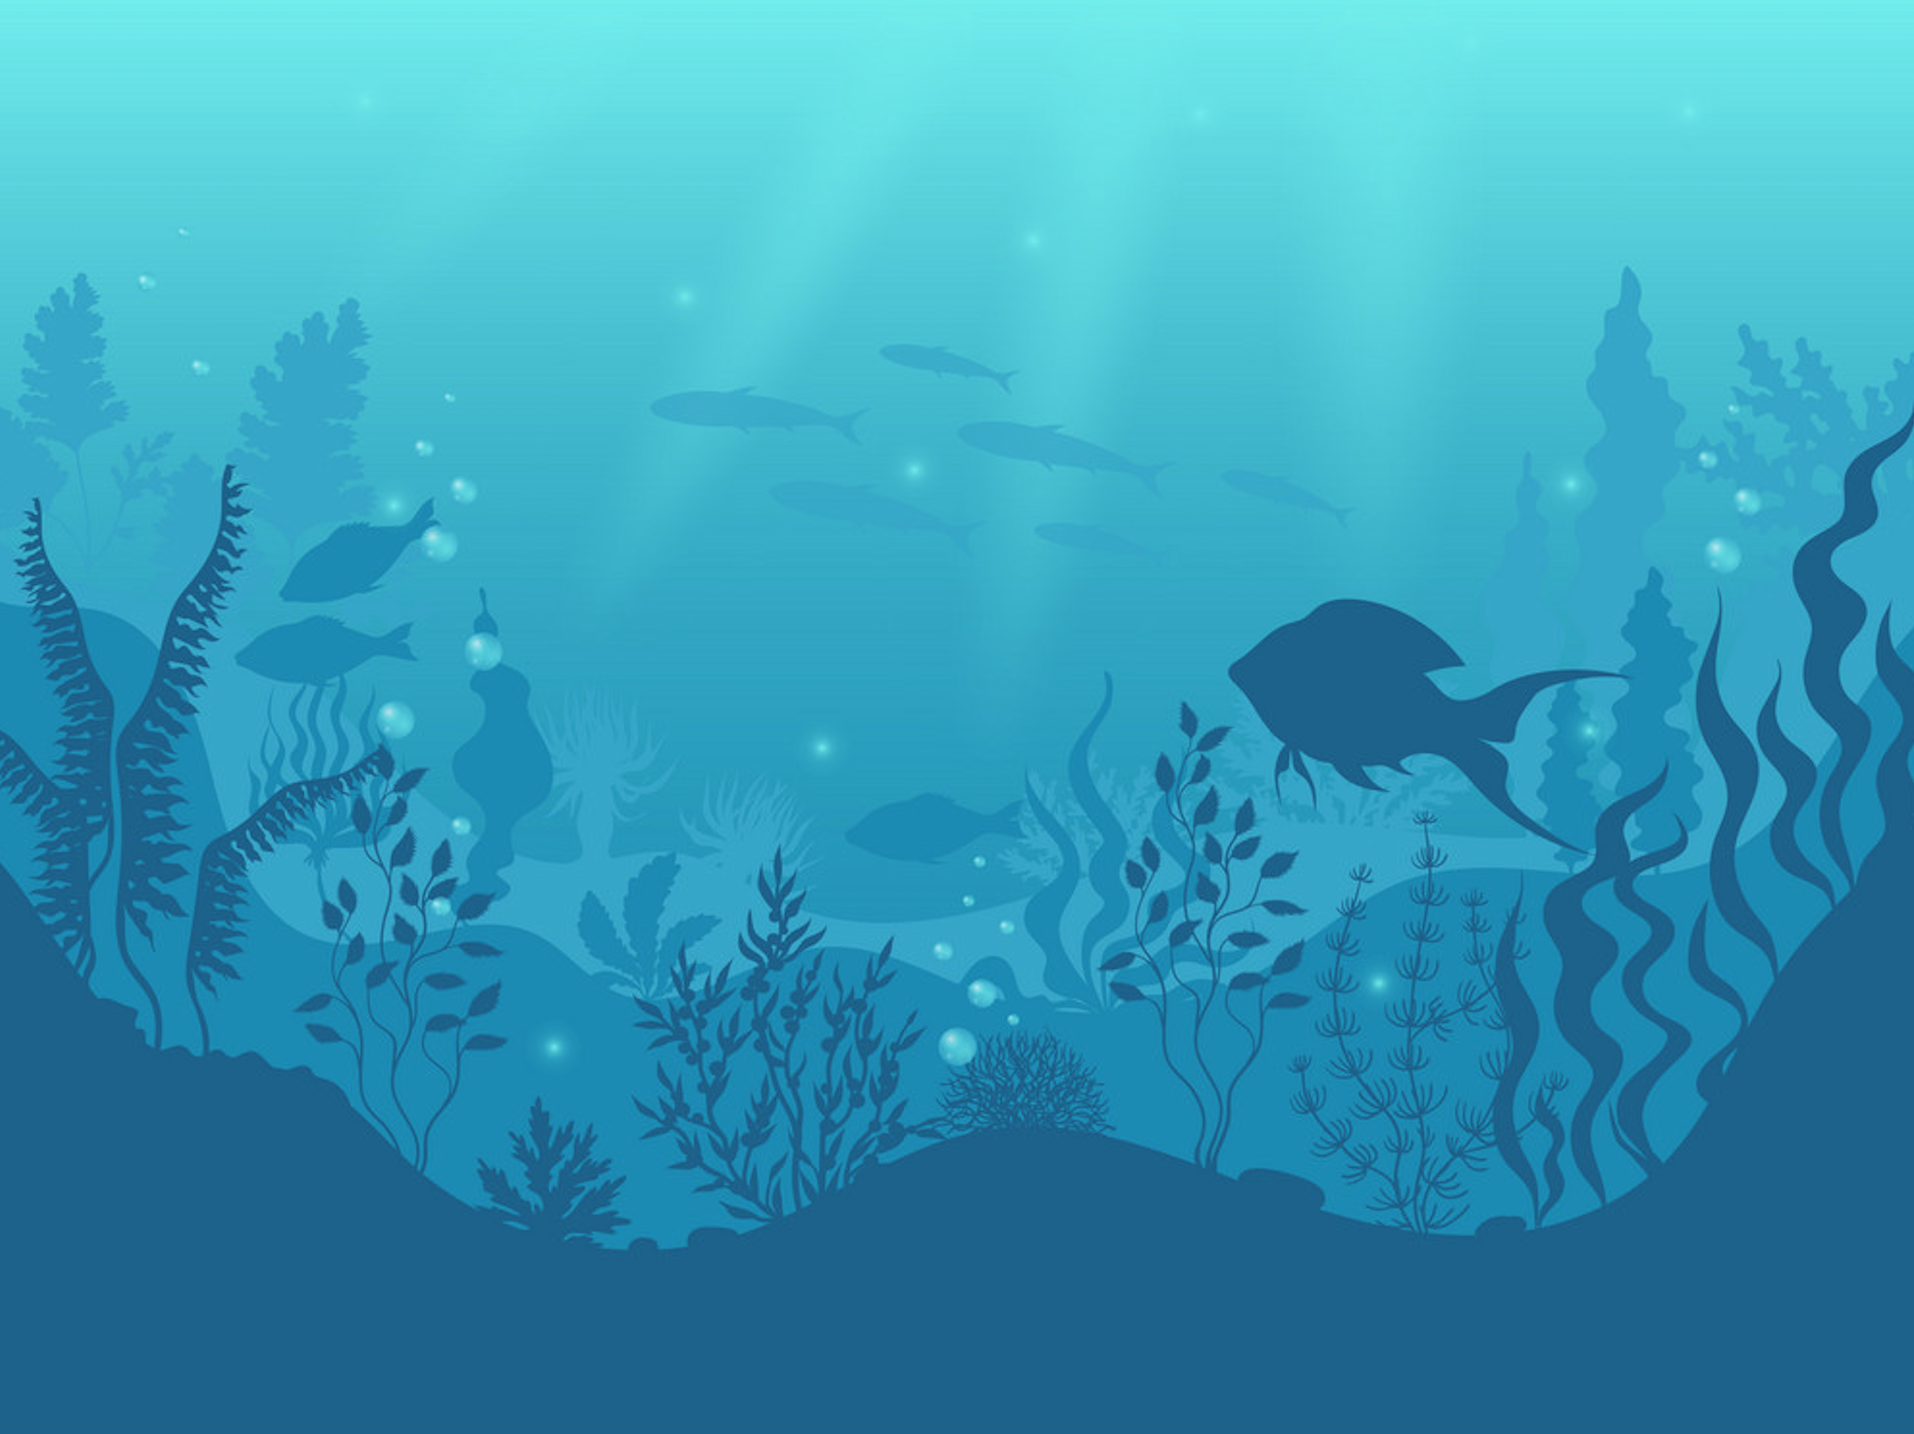
\includegraphics[keepaspectratio=true,width=0.85\paperwidth,overlay]{Images/sea.png}
\end{frame}

% \begin{frame}{\huge{Learning from experience,\\ 
% Exploring the sea}}
%     * Exploring the sea. Diving with a hose\\
%     Good morning. I was a little older than you when I had the idea 
    
    
%     % * Bottle with holes different lengths of water beam. Show picture water rocket.\\
    
%     % * How animals feet adapt to environment.\\ 
    
%     % Concept of pressure is needed to explain many different physical situations and processes.
    
%     % By the end of this Unit (not lesson) you will be able to understand all this phenomena in terms of pressure and forces
    
%     \textbf{Have you ever tried something like that?}
% \end{frame}


\begin{frame}
\titlepage
\end{frame}




\begin{frame}{\huge{Is pressure the same as force?}}
%Force and pressure the same thing?

{\huge Would you rather\dots? two options}
\begin{table}[H]
    \centering
    \scalebox{1}{
    \begin{tabular}{|l||l|}\hline
     \cellcolor{yellow} \textbf{A}    & \cellcolor{yellow}   \textbf{B} \\\hline
    %  \textbf{breathe} through a 2 m tube & \textbf{breathe} at the beach near the  \\
    %  to the surface under 1.5 m of & ocean.\\
    %  water in the ocean. & \\\hline
     \textbf{have} someone wearing cleats & \textbf{have} someone wearing tennis.\\
     step on your foot. & shoes step on your foot. \\\hline\hline
     \textbf{have} an elephant stand on & \textbf{have} an elephant balance on a \\
     your foot directly. & drawing pin on top of your foot.   \\\hline
    %  \textbf{consider} pressure and force  & \textbf{consider} force and pressure  \\
    %  just as forces of different type.  & totally different quantities.\\\hline
    \end{tabular}}
\end{table}

\centering 
{\huge You chose to minimize the pressure!}\\

\centering 
{\huge Same force was applied!}\\

\vspace{1cm}
\centering 
\textcolor{gray!40}{\Large Intuitive explanation Pressure $\ne$ Force. Balloon!}

\end{frame}






\begin{frame}{\huge{Today's Learning objectives}}
   \begin{itemize}
   \item[\bf{(1)}] \textbf{To appreciate the importance and universality of the concept of pressure.}
   \item[\bf{(2)}] \textbf{To understand that real application of forces imply surface contact.}
   \item[\bf{(3)}] \textbf{Be able to explain how force distributes over area rather than a point when applied over a surface.}
   \item[\bf{(4)}] \textbf{Be able to calculate the pressure given the force and the area of the surface.}
   
    %   \item[(1)] Recall the concept of force.
    %   \item[(2)] Contact forces act through surface contact.
    %   \item[(3)] Forces don't act locally. 
    %   \item[(4)] Forces distribute over the surface (area).
    %   \item[(5)] Definition of pressure.
   \end{itemize}
\end{frame}






\begin{frame}{\huge{Universality and importance: Solid}}% of pressure
%   \begin{itemize}
%       \item[] \textbf{Pressure in solids}
% \end{itemize}
\textcolor{red}{Objects designed to \textbf{increase} pressure and go through other solids}
\begin{itemize}
\item[]
       \begin{figure}
           \centering
           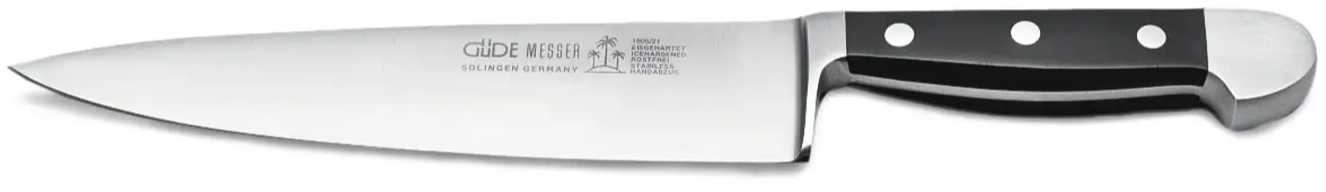
\includegraphics[scale=0.4]{Images/knife.png}
       \end{figure}
       \begin{figure}
           \centering
           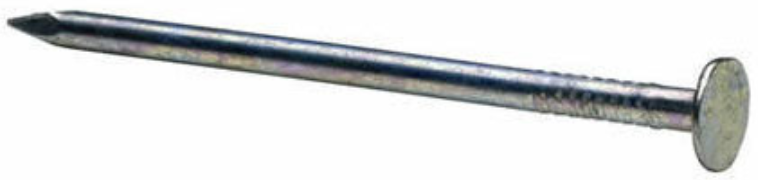
\includegraphics[scale=0.4]{Images/nail.png}\hspace{1cm}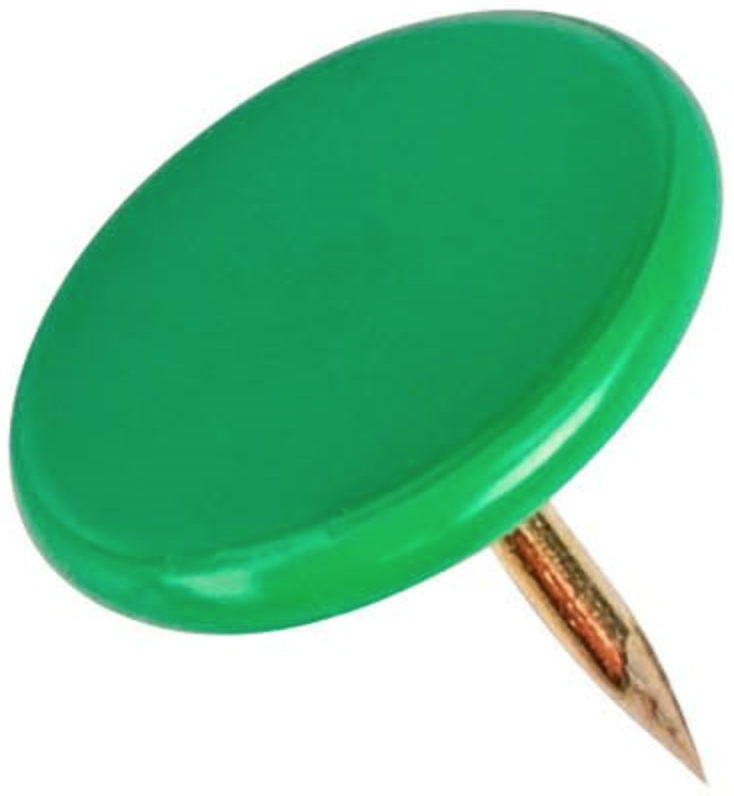
\includegraphics[scale=0.1]{Images/pin.png}
       \end{figure}
       %\item Knife, nails, pins,\dots % force lense focalizes force.
       \end{itemize}
       \textcolor{red}{Objects designed to \textbf{decrease} the pressure and reduce sinkage}
      \begin{itemize}
\item[]
       \begin{figure}
           \centering
           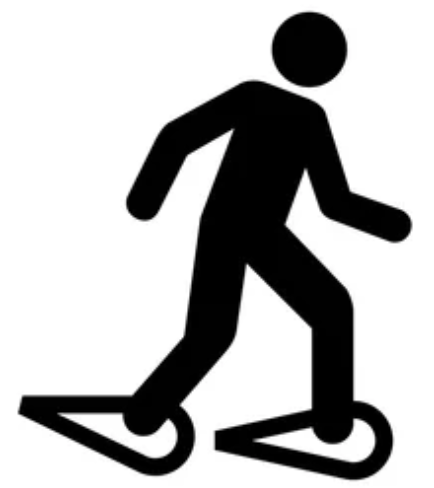
\includegraphics[scale=0.3]{Images/snow_racket_2.png}\hspace{0.3cm}
           %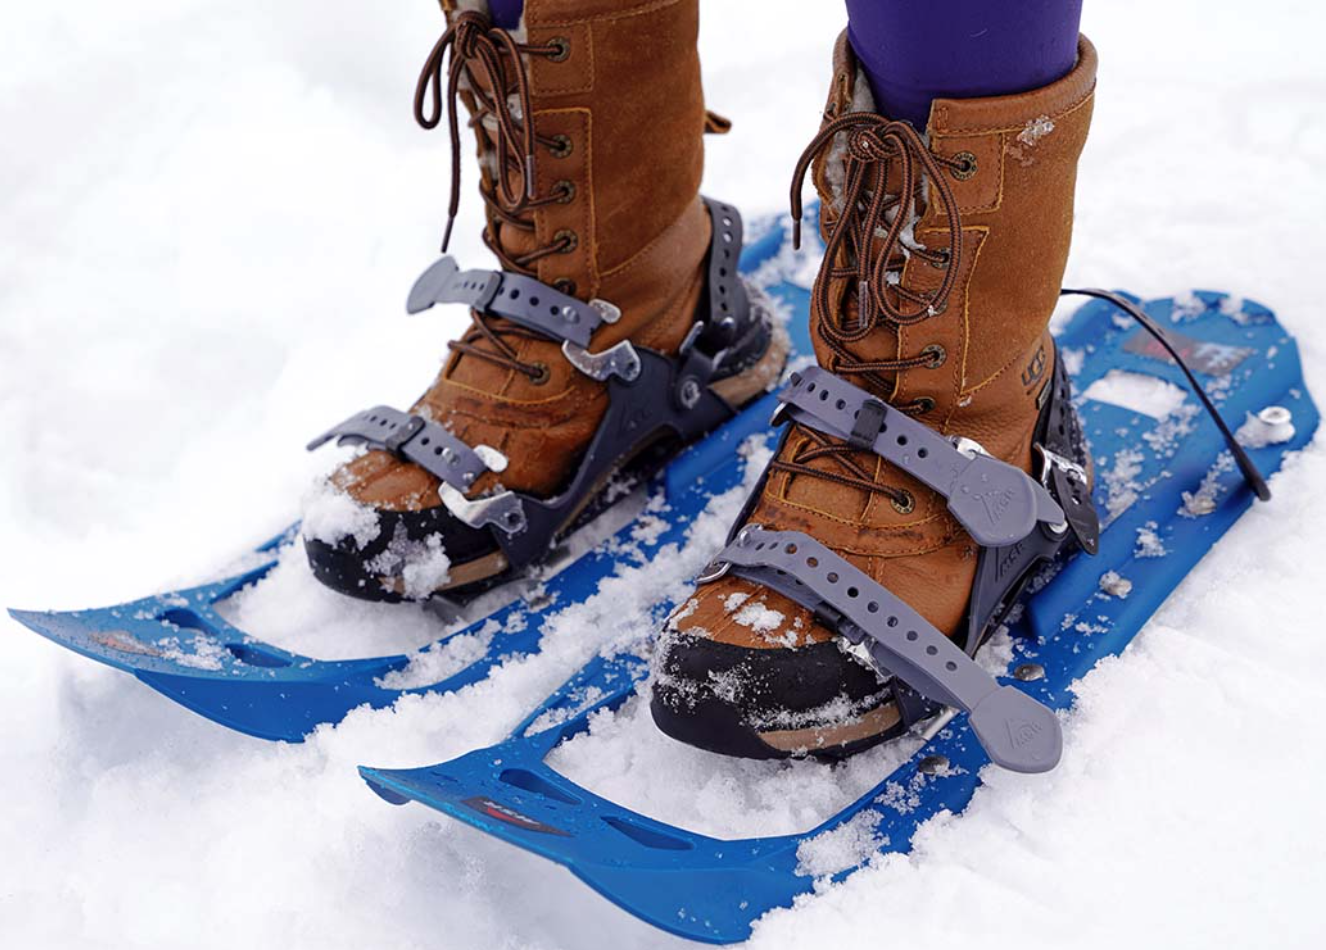
\includegraphics[scale=0.15]{Images/snow_racket.png}
           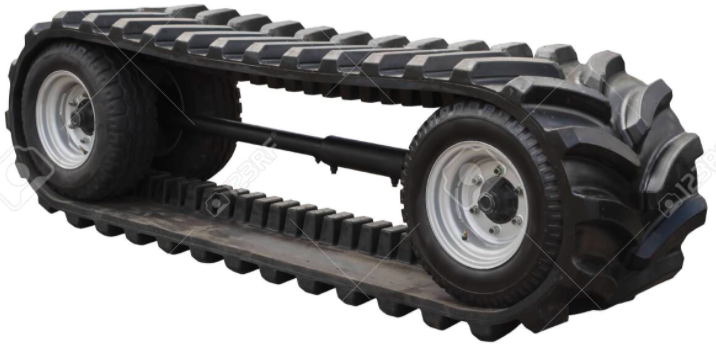
\includegraphics[scale=0.27]{Images/caterpillar_wheels.png}\hspace{0.3cm}
           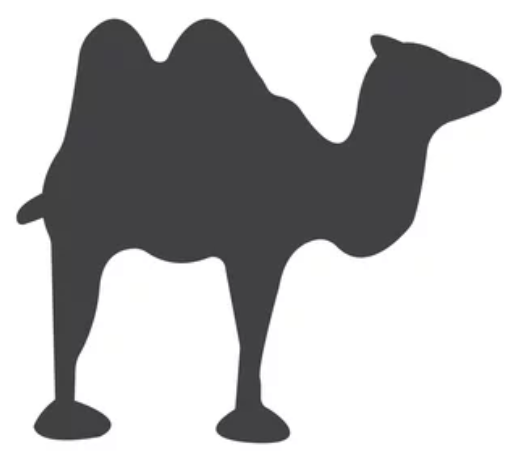
\includegraphics[scale=0.3]{Images/camel_foot_2.png}
       \end{figure}
       %\item Knife, nails, pins,\dots % force lense focalizes force.
       \end{itemize}
%       \begin{itemize}
%         \item[]
       
%       \item Walking on snow, sand, mud, \dots  Snow rackets, Skis to reduce sinkage. Animal adaption.
       
       
      
       
       
%     %\item Building foundations.
%       \item[] \textbf{Liquids}
%       \item Tap pressure.
%       \item Blood pressure.
%       \item Hydraulic press. Force multiplier. Brakes, Cranes, lift.
%       \item[] \textbf{Gases}
%       \item Tyre pressure.
%       \item Atmospheric pressure. Good \& Bad weather.
%       \item[] Combination
%   \end{itemize}
\end{frame}





\begin{frame}{\huge{Universality and importance: Liquid}}% of pressure
   \begin{itemize}
       %\item[] \textbf{Pressure in Liquids}
       \item Tap water pressure.
    %   \begin{figure}
    %       \centering
    %       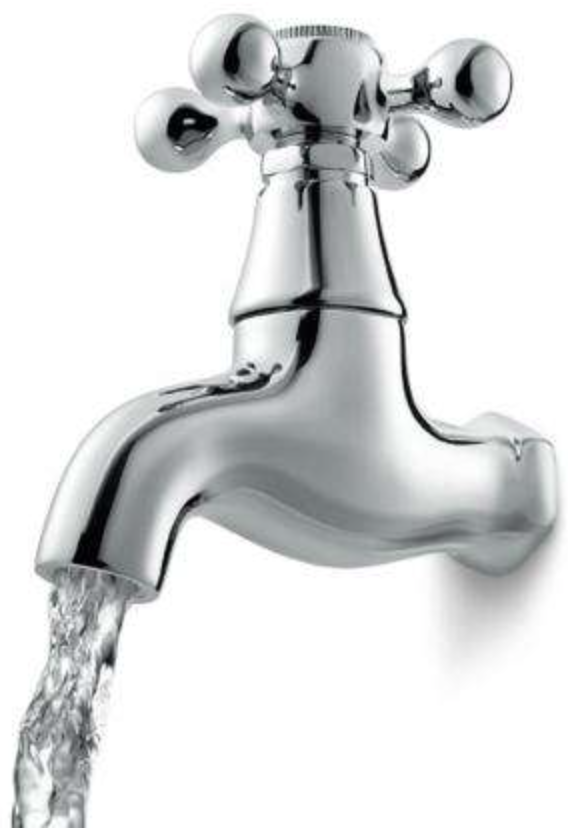
\includegraphics[scale=0.3]{Images/tap.png}
    %   \end{figure}
       \item Blood pressure.
       \item Hydraulic press. Brakes, cranes, lifts. Force multiplier.
   \end{itemize}
      \begin{figure}
          \centering
          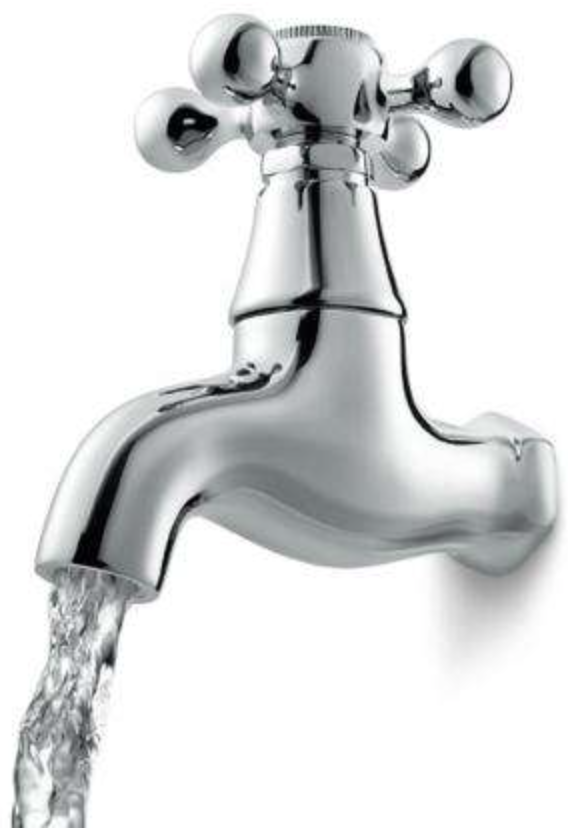
\includegraphics[scale=0.2]{Images/tap.png}
          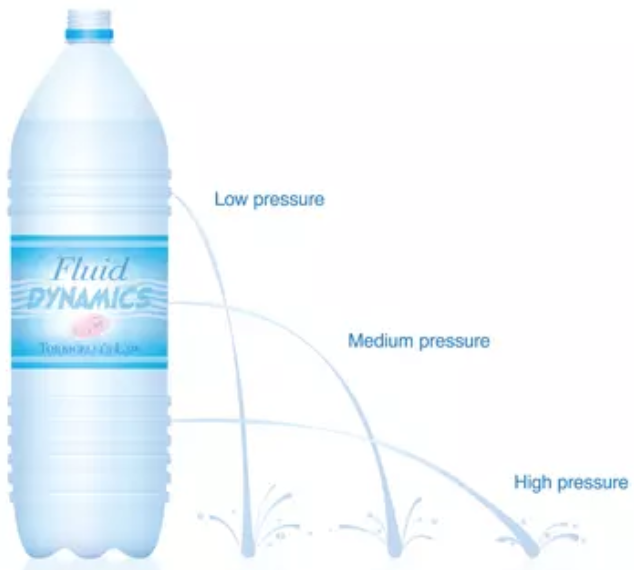
\includegraphics[scale=0.35]{Images/bottle_holes.png}
          
\includegraphics[scale=0.2]{Images/blood_pressure.png}
      \end{figure}
%   \begin{tikzpicture}[remember picture,overlay]
%     \node[xshift=65mm,yshift=-48mm,anchor=north west] at (current page.north east){%
%     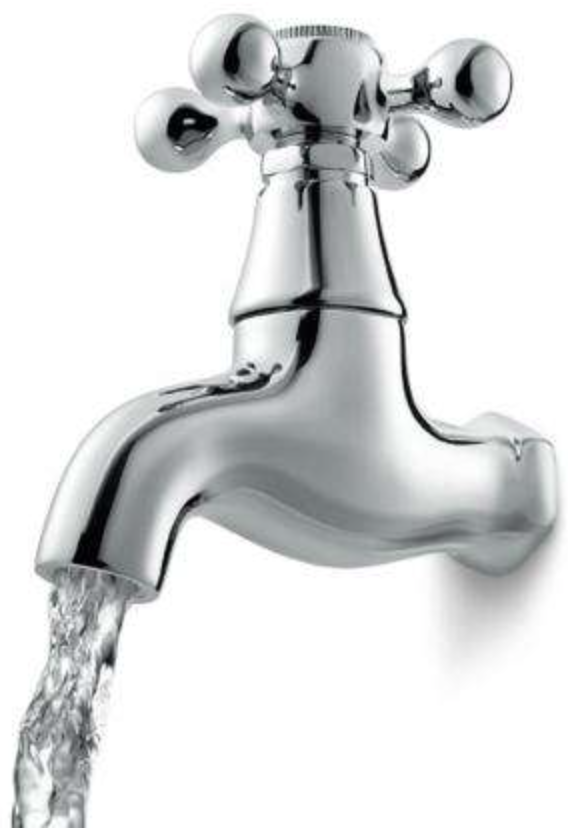
\includegraphics[scale=0.3]{Images/tap.png}};
% \end{tikzpicture}
\end{frame}














\begin{frame}{\huge{Universality and importance: Gas}}% of pressure
   \begin{itemize}
       %\item[] \textbf{Pressure in Liquids}
       \item Pressurized gas in different containers.
       \item Atmospheric pressure. Weather forecast. High \& Low pressures.
   \end{itemize}
      \begin{figure}
          \centering
         
         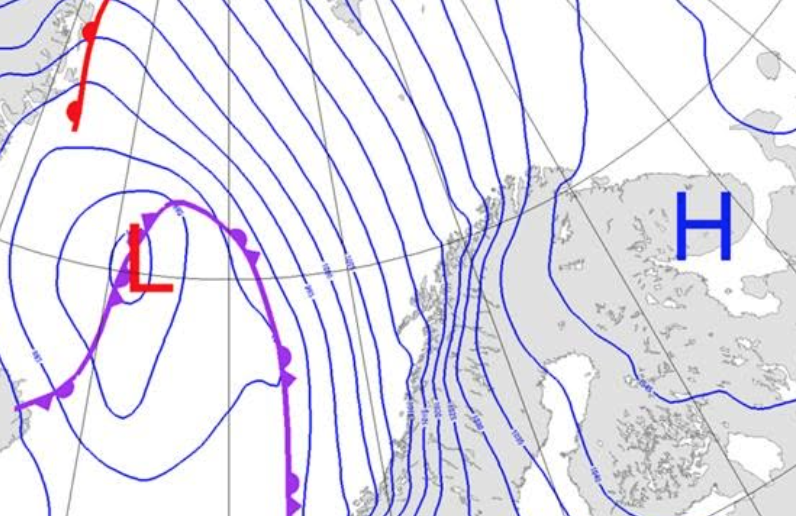
\includegraphics[scale=0.35]{Images/isobaric_map.png}
        %   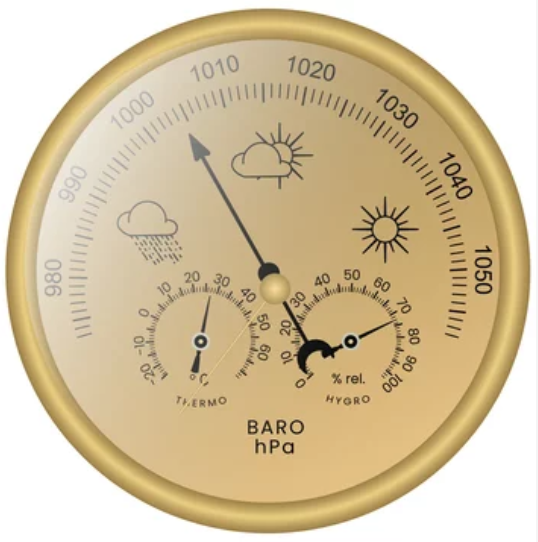
\includegraphics[scale=0.35]{Images/barometer.png}
          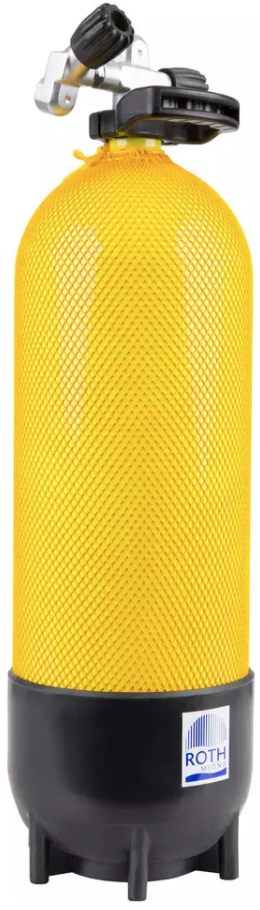
\includegraphics[scale=0.25]{Images/diving_tank.png}
          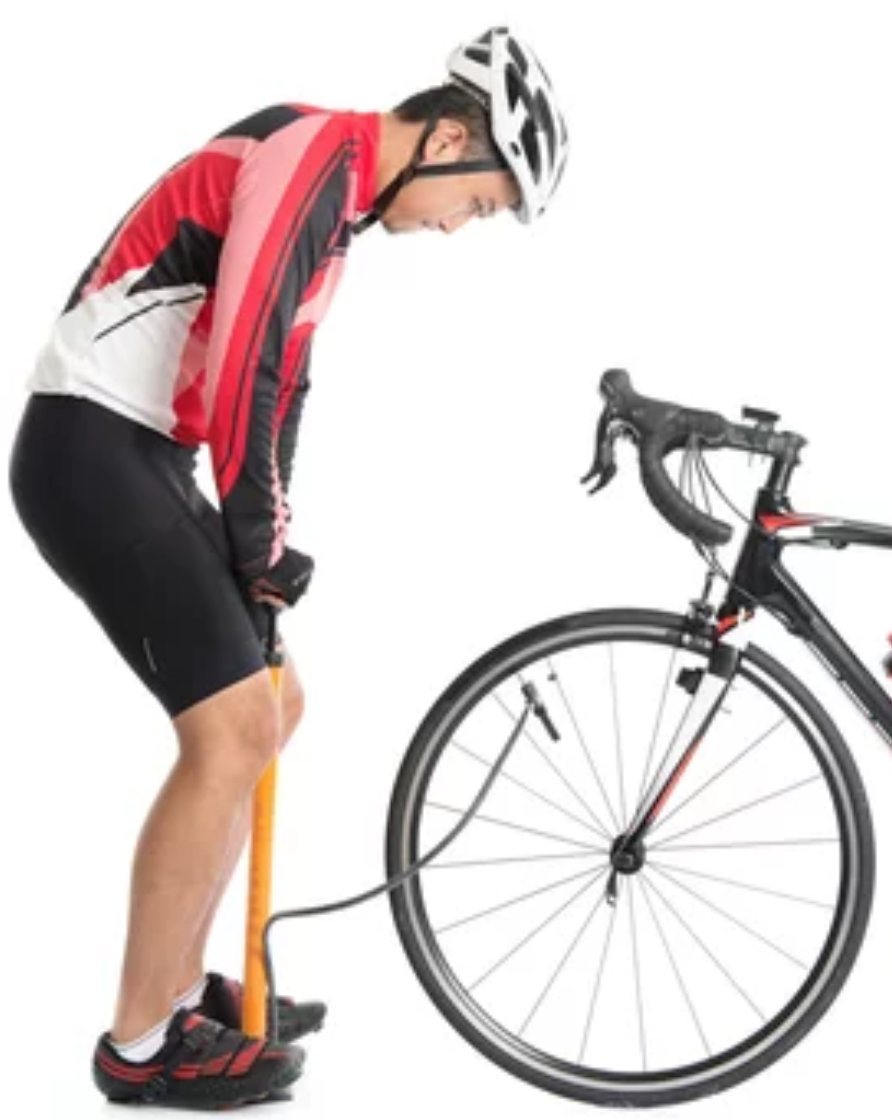
\includegraphics[scale=0.2]{Images/tyre_bicycle.png}
        %   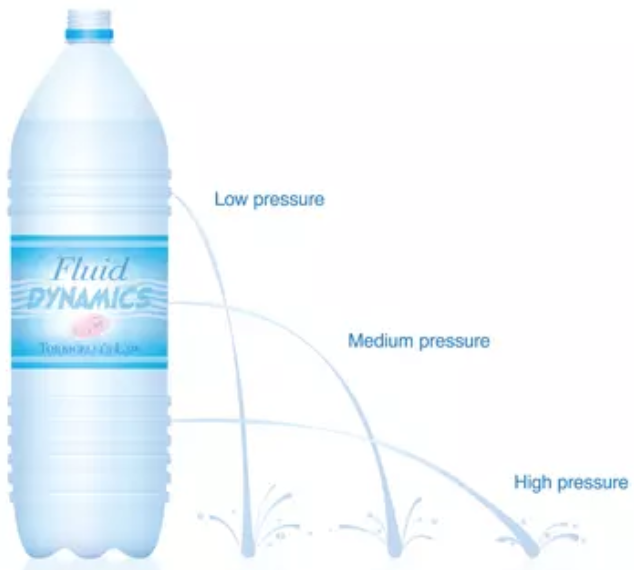
\includegraphics[scale=0.35]{Images/bottle_holes.png}
        %   
\includegraphics[scale=0.2]{Images/blood_pressure.png}
      \end{figure}
%   \begin{tikzpicture}[remember picture,overlay]
%     \node[xshift=65mm,yshift=-48mm,anchor=north west] at (current page.north east){%
%     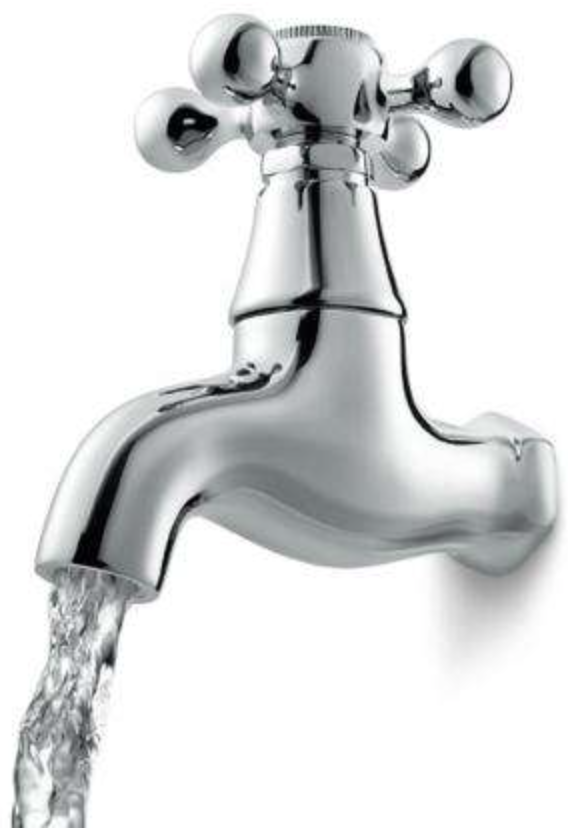
\includegraphics[scale=0.3]{Images/tap.png}};
% \end{tikzpicture}
\end{frame}

















% \begin{frame}{\huge{Geometry of the objects}}
%     The message is that pressure is an important concept that appears in many different contexts and natural processes. In this sense pressure is universal.
% \end{frame}




% \begin{frame}{Frame Title}


% % \documentclass[12pt]{article}
% % \usepackage{tikz}
% % \usetikzlibrary{positioning}
% % \begin{document}
% % \pagestyle{empty}


% \begin{tikzpicture}[scale=.6,every node/.style={minimum size=1cm},on grid]
		
%     %slanting: production of a set of n 'laminae' to be piled up. N=number of grids.
%     \begin{scope}[
%             yshift=-83,every node/.append style={
%             yslant=0.5,xslant=-1},yslant=0.5,xslant=-1
%             ]
%         % opacity to prevent graphical interference
%         \fill[white,fill opacity=0.9] (0,0) rectangle (5,5);
%         \draw[step=4mm, black] (0,0) grid (5,5); %defining grids
%         \draw[step=1mm, red!50,thin] (3,1) grid (4,2);  %Nested Grid
%         \draw[black,very thick] (0,0) rectangle (5,5);%marking borders
%         \fill[red] (0.05,0.05) rectangle (0.35,0.35);
%         %Idem as above, for the n-th grid:
%     \end{scope}
    	
%     \begin{scope}[
%     	yshift=0,every node/.append style={
%     	    yslant=0.5,xslant=-1},yslant=0.5,xslant=-1
%     	             ]
%         \fill[white,fill opacity=.9] (0,0) rectangle (5,5);
%         \draw[black,very thick] (0,0) rectangle (5,5);
%         \draw[step=5mm, black] (0,0) grid (5,5);
%     \end{scope}
    	
%     \begin{scope}[
%     	yshift=90,every node/.append style={
%     	yslant=0.5,xslant=-1},yslant=0.5,xslant=-1
%     	             ]
%     	\fill[white,fill opacity=.9] (0,0) rectangle (5,5);
%     	\draw[step=10mm, black] (1,1) grid (4,4);
%     	\draw[black,very thick] (1,1) rectangle (4,4);
%     	\draw[black,dashed] (0,0) rectangle (5,5);
%     \end{scope}
    	
%     \begin{scope}[
%     	yshift=170,every node/.append style={
%     	    yslant=0.5,xslant=-1},yslant=0.5,xslant=-1
%     	  ]
%         \fill[white,fill opacity=0.6] (0,0) rectangle (5,5);
%         \draw[step=10mm, black] (2,2) grid (5,5);
%         \draw[step=2mm, green] (2,2) grid (3,3);
%         \draw[black,very thick] (2,2) rectangle (5,5);
%         \draw[black,dashed] (0,0) rectangle (5,5);
%     \end{scope}
    	
%     \begin{scope}[
%         yshift=-170,every node/.append style={
%         yslant=0.5,xslant=-1},yslant=0.5,xslant=-1
%                   ]
%         %marking border
%         \draw[black,very thick] (0,0) rectangle (5,5);

%       	%drawing corners (P1,P2, P3): only 3 points needed to define a plane.
%         \draw [fill=lime](0,0) circle (.1) ;
%         \draw [fill=lime](0,5) circle (.1);
%         \draw [fill=lime](5,0) circle (.1);
%         \draw [fill=lime](5,5) circle (.1);

%         %drawing bathymetric hypotetic countours on the bottom grid:    	
%         \draw [ultra thick](0,1) parabola bend (2,2) (5,1)  ;
%         \draw [dashed] (0,1.5) parabola bend (2.5,2.5) (5,1.5) ;
%         \draw [dashed] (0,2) parabola bend (2.7,2.7) (5,2)  ;
%         \draw [dashed] (0,2.5) parabola bend (3.5,3.5) (5,2.5)  ;
%         \draw [dashed] (0,3.5)  parabola bend (2.75,4.5) (5,3.5);
%         \draw [dashed] (0,4)  parabola bend (2.75,4.8) (5,4);
%         \draw [dashed] (0,3)  parabola bend (2.75,3.8) (5,3);
%         \draw[-latex,thick](2.8,1)node[right]{$\mathsf{Shoreline}$}
%                  to[out=180,in=270] (2,1.99);
%     \end{scope} %end of drawing grids

%     %putting arrows and labels:
%     \draw[-latex,thick] (6.2,2) node[right]{$\mathsf{Bathymetry}$}
%          to[out=180,in=90] (4,2);

%     \draw[-latex,thick](5.8,-.3)node[right]{$\mathsf{Comp.\ G.}$}
%         to[out=180,in=90] (3.9,-1);

%     \draw[-latex,thick](5.9,5)node[right]{$\mathsf{Wind\ G.}$}
%         to[out=180,in=90] (3.6,5);

%     \draw[-latex,thick](5.9,8.4)node[right]{$\mathsf{Friction\ G.}$}
%         to[out=180,in=90] (3.2,8);

%     \draw[-latex,thick,red](5.3,-4.2)node[right]{$\mathsf{G. Cell}$}
%         to[out=180,in=90] (0,-2.5);

%     \draw[-latex,thick,red](4.3,-1.9)node[right]{$\mathsf{Nested\ G.}$}
%         to[out=180,in=90] (2,-.5);

%     \draw[-latex,thick](4,-6)node[right]{$\mathsf{Batymetry}$}
%         to[out=180,in=90] (2,-5);	
%     %drawing points on grid's conrners.
%     \fill[black,font=\footnotesize]
%         (-5,-4.3) node [above] {$P_{1}$}
%         (-.3,-5.6) node [below] {$P_{2}$}
%         (5.5,-4) node [above] {$P_{3}$};	
% \end{tikzpicture}

% % \end{document} 

    
% \end{frame}









\begin{frame}{\huge{How real forces are applied?}}% to solids

\huge{\textbf{Point or surface?}}

\begin{figure}
    \centering
    \begin{tikzpicture}
\pgfmathsetmacro{\cubex}{3}
\pgfmathsetmacro{\cubey}{2}
\pgfmathsetmacro{\cubez}{2}
\draw[red,fill=red!20] (0,0,0) -- ++(-\cubex,0,0) -- ++(0,-\cubey,0) -- ++(\cubex,0,0) -- cycle;
\draw[red,fill=red!20] (0,0,0) -- ++(0,0,-\cubez) -- ++(0,-\cubey,0) -- ++(0,0,\cubez) -- cycle;
\draw[red,fill=red!20] (0,0,0) -- ++(-\cubex,0,0) -- ++(0,0,-\cubez) -- ++(\cubex,0,0) -- cycle;
% Vector
\draw[<-,line width=1mm] ({0.2*\cubey},{-0.3*\cubey})--(3,{-0.3*\cubey});
%\node at (2,0.2) {\huge $\bm F$};
\end{tikzpicture}
\end{figure}



\begin{figure}
    \centering
    \begin{tikzpicture}
\pgfmathsetmacro{\cubex}{3}
\pgfmathsetmacro{\cubey}{2}
\pgfmathsetmacro{\cubez}{2}
\draw[red,fill=red!20] (0,0,0) -- ++(-\cubex,0,0) -- ++(0,-\cubey,0) -- ++(\cubex,0,0) -- cycle;
\draw[red,fill=red!20] (0,0,0) -- ++(0,0,-\cubez) -- ++(0,-\cubey,0) -- ++(0,0,\cubez) -- cycle;
\draw[red,fill=red!20] (0,0,0) -- ++(-\cubex,0,0) -- ++(0,0,-\cubez) -- ++(\cubex,0,0) -- cycle;
%Ghost point
\draw[white!0] (2.9,{-0.3*\cubey})--(3,{-0.3*\cubey});
% man pushing 

%\node at (1.5,0) {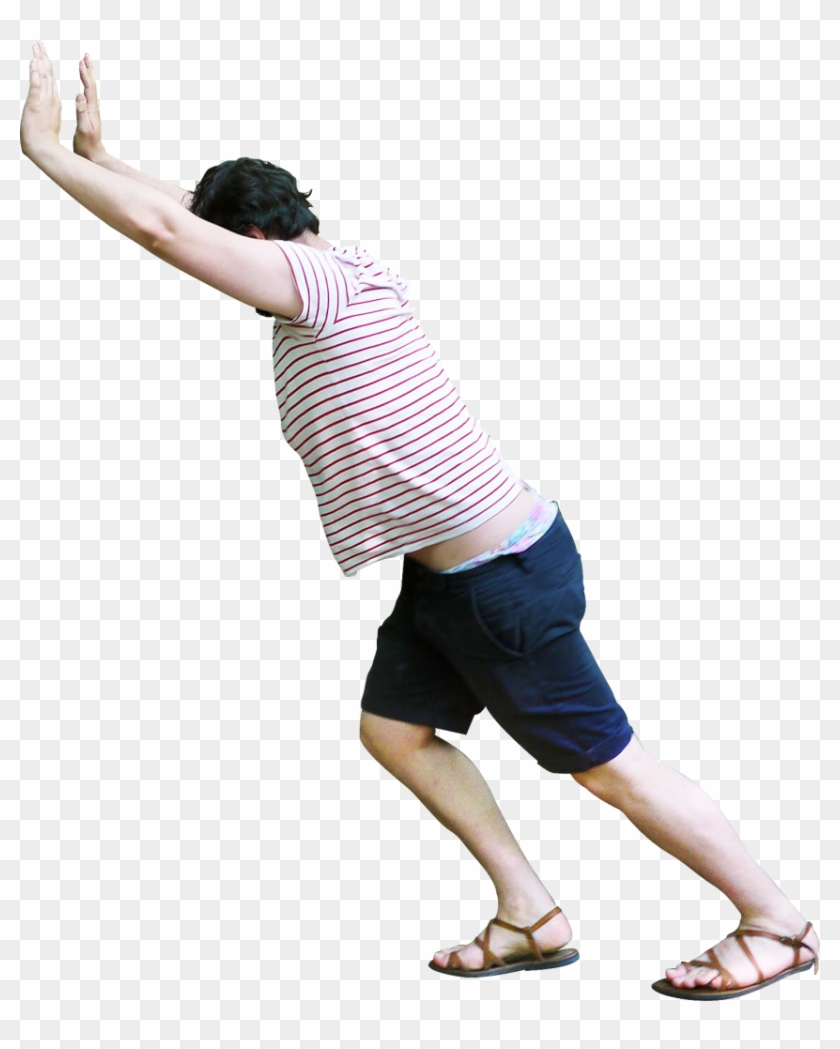
\includegraphics[scale=0.05]{Images/pushing_man.png}};

%\rput(Center)
\node at (1.7,-1.2){\special{ps: 0.4 .setopacityalpha}\reflectbox{
\includegraphics[scale=0.06]{Images/pushingmanx.png}}}
%
% \node at (2,0.2) {\huge $\bm F$};
\end{tikzpicture}
\end{figure}

\end{frame}








\begin{frame}{\huge{Contact between surfaces}}

\begin{itemize}
    \Large{\item Real \textbf{contact} between solid objects \textbf{involves  the contact of their surfaces.}}
    \item When you apply a force the force is transmitted trough the surfaces in contact.
    \item Pressure tells you about the \textbf{quantity of force} \textbf{distributed} over the surface.
\end{itemize}


%CONTACT FORCES You have studied!\\


% because of the nature of solids even applying pointy arrows force will \textbf{distribute over the surface}

% representation of a force like an arrow.

% No pointy arrows applied to a point!

% * In many cases Real application of forces involve contact of surfaces. Forces are not applied to one point. 
% * Depending on how force is applied\\
% *will have different effects on the material
% * pushing a block of butter with a knife.

\end{frame}






% %% Here mods
% \begin{frame}{\huge{Contact Area}}

% \begin{figure}
%     \centering
% \begin{tikzpicture}[scale=1.1,every node/.style={minimum size=1cm},on grid]
%     \begin{scope}[
%     	yshift=0,every node/.append style={
%     	    yslant=0.5,xslant=-1},yslant=0.5,xslant=-1
%     	             ] %,rotate=20
%         %\fill[white,fill opacity=.9] (0,0) rectangle (5,5);
%         \draw[black,very thick] (0,0) rectangle (5,5);
%         % Internal grid
%         \draw[step=5mm, black] (0,0) grid (5,5);
%         % highlighting area on grid
%         \draw[step=1mm, red!50,thin] (2,2) grid (3,3);  %Nested Grid
%         %border of nested grid
%         \draw[red,very thick] (2,2) rectangle (3,3);
%         %
%         %
%         \draw[<->,line width=0.5mm] (2,1.8)--(3,1.8);
%         \node at (2.5,1.3) {\textbf{2 m}};
        
%         \draw[<->,line width=0.5mm] (1.8,2)--(1.8,3);
%         \node[rotate=-90] at (1.3,2.5) {\textbf{2 m}};
%     \end{scope}
%     % Force draw arrow:
%     \draw[white!0,line width=0] (0,5.5)--(0,5.5);
   
    	
    
%     %putting arrows and labels:
%     %\draw[-latex,thick] (6.2,2) node[right]{$\mathsf{Surface}$} to[out=180,in=90] (4,2);

    

%     %\draw[-latex,thick,red](4.3,-1.9)node[right]{$\mathsf{Nested\ G.}$}
%     %     to[out=180,in=90] (2,-.5);
% \end{tikzpicture}
% \end{figure}
% \end{frame}












%% Here mods
\begin{frame}{\huge{Force applied over a contact area}}

\begin{figure}
    \centering
\begin{tikzpicture}[scale=1.35,every node/.style={minimum size=1cm},on grid]
    \begin{scope}[
    	yshift=0,every node/.append style={
    	    yslant=0.5,xslant=-1},yslant=0.5,xslant=-1
    	             ] %,rotate=20
        %\fill[white,fill opacity=.9] (0,0) rectangle (5,5);
        \draw[gray!50,very thick] (0.5,0.5) rectangle (4.5,4.5);
        % Internal grid
        \draw[step=5mm, gray!50] (0.5,0.5) grid (4.5,4.5);
        % red big grid
        \draw[step=5mm, red,very thick] (2,2) grid (3,3);
        % highlighting area on grid Base
        \draw[step=1mm, red!50,thin] (2,2) grid (3,3);  %Nested Grid
        %border of nested grid
        \draw[red,very thick] (2,2) rectangle (3,3);
        % Walls of object vertical lines
        % \draw[red,very thick] (2,2)--(4,4);
        % \draw[red,very thick] (2,3)--(4,5);
        % \draw[red,very thick] (3,2)--(5,4);
        % \draw[red,very thick] (3,3)--(5,5);
        % Walls of object vertical lines
        % \draw[red,very thick] (4,4)--(5,4)--(5,5)--(4,5)--(4,4);
        %
        \draw[<->,line width=0.5mm] (2,1.8)--(3,1.8);
        \node at (2.5,1.3) {\textbf{2 m}};
        
        \draw[<->,line width=0.5mm] (1.8,2)--(1.8,3);
        \node[rotate=-90] at (1.3,2.5) {\textbf{2 m}};
    \end{scope}
    % Definitions
    \node[right] at (-3.25,5) {\Large\textcolor{blue}{\textbf{Force = }$\bm F$}};
    \node[right] at (-3.25,4.5) {\Large\textcolor{red}{\textbf{Area = }$\bm A$}};
    % Force draw arrow:
    \draw[white!0,line width=0] (0,5.5)--(0,5.5);
    % Force draw arrow:
    \draw[blue,line width=1mm,->] (0,5.5)--(0,2.5);
    \node[blue,right] at (0.5,4) {\huge $\bm{F =12}$ \textbf{N}};
    % Area Label:
    \node[red,right] at (1.5,2.5) {\huge $\bm{ A=4\,}$\textbf{m}$\bm{^2}$};
    	
    %putting arrows and labels:
    %\draw[-latex,thick] (6.2,2) node[right]{$\mathsf{Surface}$} to[out=180,in=90] (4,2);

    %\draw[-latex,thick,red](4.3,-1.9)node[right]{$\mathsf{Nested\ G.}$}
    %     to[out=180,in=90] (2,-.5);
\end{tikzpicture}
\end{figure}
\end{frame}























% %% Here mods
% \begin{frame}{\huge{Area}}

% \begin{figure}
%     \centering
% \begin{tikzpicture}[scale=1.1,every node/.style={minimum size=1cm},on grid]
%     \begin{scope}[
%     	yshift=0,every node/.append style={
%     	    yslant=0.5,xslant=-1},yslant=0.5,xslant=-1
%     	             ] %,rotate=20
%         %\fill[white,fill opacity=.9] (0,0) rectangle (5,5);
%         \draw[black,very thick] (0,0) rectangle (5,5);
%         % Internal grid
%         \draw[step=5mm, black] (0,0) grid (5,5);
%         % highlighting area on grid
%         \draw[step=1mm, red!50,thin] (2,2) grid (3,3);  %Nested Grid
%         %border of nested grid
%         \draw[red,very thick] (2,2) rectangle (3,3);
%     \end{scope}
%     % Force draw arrow:
%     \draw[blue,line width=1mm,->] (0,5.5)--(0,2.5);
%     \node[blue] at (0.5,4) {\huge $\bm F$};
%     % Area Label:
%     \node[red] at (1.5,2.5) {\huge $\bm A$};
    	
    
%     %putting arrows and labels:
%     %\draw[-latex,thick] (6.2,2) node[right]{$\mathsf{Surface}$} to[out=180,in=90] (4,2);

    

%     %\draw[-latex,thick,red](4.3,-1.9)node[right]{$\mathsf{Nested\ G.}$}
%     %     to[out=180,in=90] (2,-.5);
% \end{tikzpicture}
% \end{figure}
% \end{frame}
















% \begin{frame}{\huge{Force applied over a surface}}

% \begin{figure}
%     \centering
% \begin{tikzpicture}[scale=1.1,every node/.style={minimum size=1cm},on grid]
%     \begin{scope}[
%     	yshift=0,every node/.append style={
%     	    yslant=0.5,xslant=-1},yslant=0.5,xslant=-1
%     	             ] %,rotate=20
%         %\fill[white,fill opacity=.9] (0,0) rectangle (5,5);
%         \draw[black,very thick] (0,0) rectangle (5,5);
%         % Internal grid
%         \draw[step=5mm, black] (0,0) grid (5,5);
%         % highlighting area on grid
%         \draw[step=1mm, red!50,thin] (2,2) grid (3,3);  %Nested Grid
%         %border of nested grid
%         \draw[red,very thick] (2,2) rectangle (3,3);
%     \end{scope}
%     % Force draw arrow:
%     \draw[blue,line width=1mm,->] (0,5.5)--(0,2.5);
%     \node[blue,right] at (0.5,4) {\huge $\bm{ F=12\,}$\textbf{N}};
%     % Area Label:
%     \node[red,right] at (1.5,2.5) {\huge $\bm{ A=4\,}$\textbf{m}$\bm{^2}$};
    	
    
%     %putting arrows and labels:
%     %\draw[-latex,thick] (6.2,2) node[right]{$\mathsf{Surface}$} to[out=180,in=90] (4,2);

    

%     %\draw[-latex,thick,red](4.3,-1.9)node[right]{$\mathsf{Nested\ G.}$}
%     %     to[out=180,in=90] (2,-.5);
% \end{tikzpicture}
% \end{figure}
% \end{frame}

















\begin{frame}{\huge{Distributing the force over area}}

% \begin{itemize}
%     \item[\bf (1)] Even distribution:\\
%     We want to give a share of force to each of a number of area units.
%     \item[\bf (2)] Force = 12 N and Area = 4 m$^2$
% \end{itemize}

\Large{An \textbf{even distribution} of the force over the area}\\
\Large{results in a force of \textbf{3 N per square metre}.}

\begin{figure}
    \centering
\begin{tikzpicture}[scale=1.1,every node/.style={minimum size=1cm},on grid]
    % Force draw arrow:
    \draw[blue,line width=1mm,->] (0,5.5)--(0,2.5);
    \node[blue,right] at (0.5,4) {\huge $\bm{12\,}$\textbf{N =}};
    % Small forces
    \draw[Green,line width=1mm,->] (3.2,5.5)--(3.2,4.75);
    \node[Green,right] at (3.7,{5.5-0.375}) {\huge $\bm{ 3\,}$\textbf{N}};
    
    \draw[Green,line width=1mm,->] (3.2,4.75)--(3.2,4.0);
    \node[Green,right] at (3.7,{4.75-0.375}) {\huge $\bm{ 3\,}$\textbf{N}};
    
    \draw[Green,line width=1mm,->] (3.2,4.0)--(3.2,3.25);
    \node[Green,right] at (3.7,{4.0-0.375}) {\huge $\bm{ 3\,}$\textbf{N}};
    
    \draw[Green,line width=1mm,->] (3.2,3.25)--(3.2,2.5);
    \node[Green,right] at (3.7,{3.25-0.375}) {\huge $\bm{ 3\,}$\textbf{N}};
    
    % dashed gray lines to visualize same scale
    \draw[dashed,gray] (0,5.5)--(3.2,5.5);
    \draw[dashed,gray] (0,2.5)--(3.2,2.5);
    
    % Sum of distribution.
    %\node[black,right] at (4.75,4) {\huge \textbf{= 2 N+2 N+2 N+2 N}};
   
\end{tikzpicture}
\end{figure}
\end{frame}














\begin{frame}{\huge{Replace force by pressure}}

% \centering
%     \textbf{\Large The force distributed over area is the pressure!}

\begin{figure}
    \centering
\begin{tikzpicture}[scale=1.35,every node/.style={minimum size=1cm},on grid]
    \begin{scope}[
    	yshift=0,every node/.append style={
    	    yslant=0.5,xslant=-1},yslant=0.5,xslant=-1
    	             ] %,rotate=20
        %\fill[white,fill opacity=.9] (0,0) rectangle (5,5);
        \draw[gray!50,very thick] (0.5,0.5) rectangle (4.5,4.5);
        % Internal grid
        \draw[step=5mm, gray!50] (0.5,0.5) grid (4.5,4.5);
        % red big grid
        \draw[step=5mm, red,very thick] (2,2) grid (3,3);
        % highlighting area on grid Base
        \draw[step=1mm, red!50,thin] (2,2) grid (3,3);  %Nested Grid
        %border of nested grid
        \draw[red,very thick] (2,2) rectangle (3,3);
        % Walls of object vertical lines
        % \draw[red,very thick] (2,2)--(4,4);
        % \draw[red,very thick] (2,3)--(4,5);
        % \draw[red,very thick] (3,2)--(5,4);
        % \draw[red,very thick] (3,3)--(5,5);
        % Walls of object vertical lines
        % \draw[red,very thick] (4,4)--(5,4)--(5,5)--(4,5)--(4,4);
        %
        % \draw[<->,line width=0.5mm] (2,1.8)--(3,1.8);
        % \node at (2.5,1.3) {\textbf{2 m}};
        
        % \draw[<->,line width=0.5mm] (1.8,2)--(1.8,3);
        % \node[rotate=-90] at (1.3,2.5) {\textbf{2 m}};
    \end{scope}
    % Force draw arrow:
    \draw[white!0,line width=0] (0,5.5)--(0,5.5);
    % % Force draw arrow:
    % \draw[blue,line width=1mm,->] (0,5.5)--(0,2.5);
    % \node[blue,right] at (0.5,4) {\huge $\bm{F =12}$ \textbf{N}};
    % Area Label:
    % \node[red,right] at (1.5,2.5) {\huge $\bm{ A=4\,}$\textbf{m}$\bm{^2}$};
    
    % Pressure distribution:
    \draw[Green,line width=1mm,->] (-0.5,3.25)--(-0.5,2.5); %left
    \draw[Green,line width=1mm,->] (0.5,3.25)--(0.5,2.5); %right
    \draw[Green,line width=1mm,->] (0.0,3.5)--(0.0,2.75); %top
    \draw[Green,line width=1mm,->] (0.0,3.0)--(0.0,2.25); %down
    % pressure
    \node[Green] at (0,4) {\huge $\bm{ p=3\,}$\textbf{N/m}$\bm{^2}$};
    	
    %putting arrows and labels:
    %\draw[-latex,thick] (6.2,2) node[right]{$\mathsf{Surface}$} to[out=180,in=90] (4,2);

    %\draw[-latex,thick,red](4.3,-1.9)node[right]{$\mathsf{Nested\ G.}$}
    %     to[out=180,in=90] (2,-.5);
\end{tikzpicture}
\end{figure}

\end{frame}















% % Animation between force and pressure???
% \begin{frame}{\huge{Replace force by pressure}}

% \begin{figure}
%     \centering
% \begin{tikzpicture}[scale=1.1,every node/.style={minimum size=1cm},on grid]
%     \begin{scope}[
%     	yshift=0,every node/.append style={
%     	    yslant=0.5,xslant=-1},yslant=0.5,xslant=-1
%     	             ] %,rotate=20
%         %\fill[white,fill opacity=.9] (0,0) rectangle (5,5);
%         \draw[black!30,very thick] (0,0) rectangle (5,5);
%         % Internal grid 
%         \draw[step=5mm, black!30] (0,0) grid (5,5);
%         % highlighting area on grid
%         \draw[step=1mm, red!50,thin] (2,2) grid (3,3);  %Nested Grid
%         %border of nested grid
%         \draw[red,very thick] (2,2) rectangle (3,3);
%     \end{scope}
%     % Pressure distribution:
%     \draw[Green,line width=1mm,->] (-0.5,3.25)--(-0.5,2.5); %left
%     \draw[Green,line width=1mm,->] (0.5,3.25)--(0.5,2.5); %right
%     \draw[Green,line width=1mm,->] (0.0,3.5)--(0.0,2.75); %top
%     \draw[Green,line width=1mm,->] (0.0,3.0)--(0.0,2.25); %down
    
    
    
%     %\node[blue,right] at (0.5,4) {\huge $\bm{ F=8\,}$\textbf{N}};
%     % Area Label:
%     \node[red,right] at (1.5,2.5) {\huge $\bm{ A=4\,}$\textbf{m}$\bm{^2}$};
%     \node[Green] at (0,4) {\huge $\bm{ p=3\,}$\textbf{N}/\textbf{m}$\bm{^2}$};
    	
    
%     %putting arrows and labels:
%     %\draw[-latex,thick] (6.2,2) node[right]{$\mathsf{Surface}$} to[out=180,in=90] (4,2);

    

%     %\draw[-latex,thick,red](4.3,-1.9)node[right]{$\mathsf{Nested\ G.}$}
%     %     to[out=180,in=90] (2,-.5);
    
%     % Ghost points:
% %    Force draw arrow:
%     \draw[white!0] (0,5.5)--(0,5.49);
% \end{tikzpicture}
% \end{figure}
% \centering
% \textbf{\Large The force distributed over area is the pressure!}

% \end{frame}








\begin{frame}{\huge{How did we get the pressure?}}

%How pressure is obtained

\begin{itemize}
    \item[\Large \bf (1)] \Large{Identify the \textbf{surface} in \textbf{contact}.}
    \item[\bf (2)] Identify what is \textbf{the force applied to the surface}.
    \item[\bf (3)] Calculate the \textbf{quantity of surface} (area).
    \item[\bf (4)] \textcolor{red}{\textbf{Distribute evenly the force over the area}.}
    \begin{equation*}
    \boxed{\text{\textcolor{Green}{\bf Pressure}}=\frac{\text{\textcolor{blue}{\bf Force}}}{\text{\textcolor{red}{\bf Area}}}}
\end{equation*}
\end{itemize}
\Large{\textbf{Unit of pressure} in SI: \textbf{Pascal}, represented by \textbf{Pa} (1 Pa=1 N/m$^2$). Other units can be defined.\\

}
\end{frame}









\begin{frame}{\huge{Now you calculate the pressure!}}

\begin{figure}
    \centering
\begin{tikzpicture}[scale=1.35,every node/.style={minimum size=1cm},on grid]
    \begin{scope}[
    	yshift=0,every node/.append style={
    	    yslant=0.5,xslant=-1},yslant=0.5,xslant=-1
    	             ] %,rotate=20
        %\fill[white,fill opacity=.9] (0,0) rectangle (5,5);
        \draw[black,very thick] (0.5,0.5) rectangle (4.5,4.5);
        % Internal grid
        \draw[step=5mm, black] (0.5,0.5) grid (4.5,4.5);
        % highlighting area on Nested Grid
        \draw[step=1mm, red!50,thin] (1.5,2) grid (3.5,3);  %Nested Grid
        \draw[step=1mm, red!50,thin] (2,1.5) grid (3,2);  %Nested Grid
        \draw[step=1mm, red!50,thin] (2,3) grid (3,3.5);  %Nested Grid
        %
        % Red area units:
        % \draw[step=5mm, red, very thick] (1.5,1.5) grid (3.0,3.0);
        \draw[step=5mm, red, very thick] (1.5,1.5) grid (3.0,3.0);
        \draw[red, very thick] (2.5,1.5)-- (2.5,3.5);
        \draw[red, very thick] (1.5,2.5)-- (3.5,2.5);
        
        %border of nested grid
        \draw[red,very thick] (1.5,2)--(1.5,3)--(2,3)--(2,3.5)--(3,3.5)--(3,3)--(3.5,3)--(3.5,2)--(3,2)--(3,1.5)--(2,1.5)--(2,2)--(1.5,2);
    \end{scope}
    % Force draw arrow:
    \draw[blue,line width=1mm,->] (0,5.5)--(0,2.5);
    \node[blue,right] at (0.5,4) {\huge $\bm{ F=12\,}$\textbf{N}};
    % Area Label:
    \node[red,right] at (1.5,2.5) {\huge $\bm{A}$};
    	
    
    %putting arrows and labels:
    %\draw[-latex,thick] (6.2,2) node[right]{$\mathsf{Surface}$} to[out=180,in=90] (4,2);

    

    %\draw[-latex,thick,red](4.3,-1.9)node[right]{$\mathsf{Nested\ G.}$}
    %     to[out=180,in=90] (2,-.5);
\end{tikzpicture}
\end{figure}
\end{frame}












% \begin{frame}
% \frametitle{\huge{Pressure definition and units}}

% {\Large
% \begin{block}{Pressure}%Is the force applied perpendicular
% Is the force applied perpendicular to the surface of an object per unit area over which that force is \textbf{distributed}.

% \begin{equation*}
%     \text{\textcolor{Green}{\bf Pressure}}=\frac{\text{\textcolor{blue}{\bf Force}}}{\text{\textcolor{red}{\bf Area}}}
% \end{equation*}
% \end{block}}

% Different units of pressure exist. We are going to use international system of units pressure.\\

% Force / area ==> N/m$^2$ ==> Pascal, Pa

% % {\Huge
% % \begin{equation*}
% % \vec{p}=m\,\vec{v}
% % \end{equation*}}

% % \begin{itemize}
% %     \item In absence of forces there is always a {\bf Galilean transformation} where the linear momentum is equal to zero.
% % \end{itemize}

% \end{frame}












% \begin{frame}{Match with reality}
% \textbf{How this connects with reality?}

% \textbf{EXAMPLE 1} Book example

% \textbf{EXAMPLE 2} Pressure on the ground exerted by me

% (1) Identify the surface contact shoe sole - ground.
% (2) Identify the force applied to the sole my weight. 650 N
% (3) Measure the quantity of surface area of the shoe sole.\\
% (But pressure SHOW THEM THE GRAPH PAPER OF MY Shoe.)
% (4) Distribute (divide) the force over the area:

% \begin{equation*}
%     \text{\textcolor{Green}{\bf pressure}}=\frac{\text{\textcolor{blue}{\bf Force}}}{\text{\textcolor{red}{\bf Area}}}
% \end{equation*}
    
% \end{frame}







% \begin{frame}{Examples}
    
%     Please interact with me!!!
    
%     (Abstract) SHOW DIFFERENT EXAMPLES AND SOLVE THEM IN CLASS.\\
    
%     (real) Knife!\\
    
%     (Iron Nail)\\
    
    
%     * SAME FORCE AREA INCREASES!!
    
%     * SAME AREA FORCE CHANGES
    
% \end{frame}








% \begin{frame}
% \frametitle{\huge{Defining language}}

% p is the pressure.
% F is the force applied to the surface
% A is the area of the surface.

% \end{frame}















% \begin{frame}
% \frametitle{\huge{Calculating pressure}}

% \begin{block}{Equation for pressure}
% \begin{equation*}
%   \bm{\text{pressure}=\frac{\text{Force applied}}{\text{Area}}}
% \end{equation*}
% \begin{itemize}
%     \item $\bm{\vec{F}}$ is the normal (to the surface) component of the force.
%     \item $\bm p$ is the pressure. Force per unit of area.
%     \item $\bm{A}$ is the area of the surface where force is applied.
% \end{itemize}
% \end{block}
% \end{frame}








% \begin{frame}
% \frametitle{\huge{Calculating pressure}}

% \begin{block}{Equation for pressure}
% \begin{equation*}
%   \bm{p=\frac{F}{A}}
% \end{equation*}
% \begin{itemize}
%     \item $\bm{\vec{F}}$ is the normal (to the surface) component of the force.
%     \item $\bm p$ is the pressure. Force per unit of area.
%     \item $\bm{A}$ is the area of the surface where force is applied.
% \end{itemize}
% \end{block}
% \end{frame}





% \begin{frame}
% \frametitle{\huge{Calculating pressure}}




% \begin{block}{Equation for pressure}
% \begin{figure}[H]
%     \centering
%     \begin{tikzpicture}[thick,scale=1.5, every node/.style={transform shape}]
%     \draw[rounded corners=10mm,draw=black,line width = 0.75mm,fill=yellow] (0,0) -- (3,0) -- (1.5,2.5) --cycle;
%     \draw[line width = 0.5mm] (0.75,1) -- (2.25,1);
%     \node[at={(1.5,0.5)},color=black]{\Huge $p\times A$};
%     \node[at={(1.5,1.5)},color=black]{\Huge $F$};
%     \end{tikzpicture}
%     %\caption{Charge $Q$, current $I$, and time $t$ relation.}
%     \label{fig:my_label}
% \end{figure}
% \begin{itemize}
%     \item $\bm{\vec{F}}$ is the normal component of the force.
%     \item $\bm p$ is the pressure. Force per unit of area.
%     \item $\bm{A}$ is the area of the surface where force is applied.
% \end{itemize}
% \end{block}
% \end{frame}








% \begin{frame}{\huge{Properties}}

% \begin{itemize}
%     \item[(1)] Pressure is an intensive quantity (does not change with the size of the system)
%     \item[(2)] Pressure can be used as force multiplier or divider.\\
%     Examples:\\
%     * knife\\
%     * caterpilar tracks\\
% \end{itemize}

% \end{frame}


% \begin{frame}{\huge{Sinkage in snow}}

% \begin{figure}
%     \centering
%     \begin{tikzpicture}
% \begin{axis}[width=0.95\textwidth,height=0.95\textheight,
% %  title = {},  % whatever name you want
%   xlabel = {Sinkage in cm},
%   ylabel = {Pressure in kPa},
%   ymin = 0, ymax = 250,
%   minor y tick num = 1,]
%   %\addplot[blue,smooth, tension=1] table {Snow-Sinkage_cm_kPa.dat};
%   \addplot [blue,line width=0.5mm,no markers, raw gnuplot] gnuplot {
%         plot 'Snow-Sinkage_cm_kPa.dat' smooth sbezier;
%     };
%     \addplot [red,line width=0.5mm,no markers, raw gnuplot] gnuplot {
%         plot 'Sand_Sinkage_cm_kPa.dat' smooth sbezier;
%     };
% \end{axis}
% \end{tikzpicture}
%     %\caption{Alger, R. and Osborne, M. (1989)}%Alger, R. and Osborne, M. (1989). Snow characterization field data collection results (Final Report No. ACA90-85-K-002). Keweenaw Research Center, Michigan Technological University, Houghton, MI.}
% \end{figure}    
% \end{frame}



\begin{frame}{\huge{Example: Shoe sole max pressure}}

\begin{itemize}
    \item[\bf (1)] The surface in contact is my \textbf{shoe sole}.
    \item[\bf (2)] The force applied to my shoe sole is my \textbf{weight}.
    \begin{equation*}
    F=65 \textcolor{red!30}{\text{ kg}} \times 10 \textcolor{red!30}{\text{ N/m}} = 650 \textcolor{red!30}{\text{ N}}
    \end{equation*}
    \item[\bf (3)] The \textbf{area of the sole} is typically.
    \begin{equation*}
    A= 200 \textcolor{red!30}{\text{ cm}^2} = 0.02 \textcolor{red!30}{\text{ m}^2}
    \end{equation*}
    \item[\bf (4)] The pressure is just:
    \begin{equation*}
        \boxed{p=\frac{650\textcolor{red!30}{\text{ N}}}{0.02\textcolor{red!30}{\text{ m}^2}}= 33000 \textcolor{red!30}{\text{ Pa}}=33 \textcolor{red!30}{\text{ kPa}}}
    \end{equation*}
\end{itemize}

We have two feet!\\

How much would I sink using my shoes in snow?\\
\end{frame}



% https://www.pngwing.com/en/free-png-nwaan/download


\begin{frame}{\huge{Sinkage in snow}}

\begin{figure}
    \centering
    \begin{tikzpicture}
\begin{axis}[width=0.95\textwidth,height=0.95\textheight,
%  title = {},  % whatever name you want
  xlabel = {\bf \Large Sinkage in cm},
  ylabel = {\bf \Large Pressure in kPa},
  ymin = 0, ymax = 80,
  minor y tick num = 1,enlarge x limits=false]
  %\addplot[blue,smooth, tension=1] table {Snow-Sinkage_cm_kPa.dat};
  \addplot [blue,line width=0.5mm,no markers, raw gnuplot] gnuplot {
        plot 'Snow-Sinkage_cm_kPa.dat' smooth sbezier;
    };
    % Arrow
    \draw[red,dashed,->,line width=1mm] (axis cs: 0,33)--(axis cs: 20,33);
    \draw[red,dashed,->,line width=1mm] (axis cs: 20,33)--(axis cs: 20,0);
    %
    % Walking man
    \put(170,90){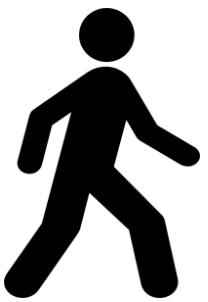
\includegraphics[scale=0.3]{Images/walking_man.png}}
    %
    %
    \node[red,right] at (axis cs: 1,75) {\bf Sinkage with normal shoes = 20 cm};
  
    %\addplot [red,line width=0.5mm,no markers, raw gnuplot] gnuplot { plot 'Sand_Sinkage_cm_kPa.dat' smooth sbezier;};
\end{axis}
\end{tikzpicture}
    %\caption{Alger, R. and Osborne, M. (1989)}%Alger, R. and Osborne, M. (1989). Snow characterization field data collection results (Final Report No. ACA90-85-K-002). Keweenaw Research Center, Michigan Technological University, Houghton, MI.}
\end{figure}    

\end{frame}









\begin{frame}{\huge{Example: Snow shoe max pressure}}

\begin{itemize}
    \item[\bf (1)] The surface in contact is my \textbf{snowshoe sole}.
    \item[\bf (2)] The force applied to my snowshoe sole is my \textbf{weight}.
    \begin{equation*}
    F=65 \textcolor{red!30}{\text{ kg}} \times 10 \textcolor{red!30}{\text{ N/m}} = 650 \textcolor{red!30}{\text{ N}}
    \end{equation*}
    \item[\bf (3)] The \textbf{area of the sole} is typically.
    \begin{equation*}
    A= 1300 \textcolor{red!30}{\text{ cm}^2} = 0.13 \textcolor{red!30}{\text{ m}^2}
    \end{equation*}
    \item[\bf (4)] The pressure is just:
    \begin{equation*}
        \boxed{p=\frac{650\textcolor{red!30}{\text{ N}}}{0.13\textcolor{red!30}{\text{ m}^2}}= 5000 \textcolor{red!30}{\text{ Pa}}=5 \textcolor{red!30}{\text{ kPa}}}
    \end{equation*}
\end{itemize}

\end{frame}












\begin{frame}{\huge{Sinkage in snow}}

\begin{figure}
    \centering
    \begin{tikzpicture}
\begin{axis}[width=0.95\textwidth,height=0.95\textheight,
%  title = {},  % whatever name you want
  xlabel = {\bf \Large Sinkage in cm},
  ylabel = {\bf \Large Pressure in kPa},
  ymin = 0, ymax = 80,
  minor y tick num = 1,enlarge x limits=false]
  %\addplot[blue,smooth, tension=1] table {Snow-Sinkage_cm_kPa.dat};
  \addplot [blue,line width=0.5mm,no markers, raw gnuplot] gnuplot {
        plot 'Snow-Sinkage_cm_kPa.dat' smooth sbezier;
    };
    % Arrow
    \draw[red,dashed,->,line width=1mm] (axis cs: 0,33)--(axis cs: 20,33);
    \draw[red,dashed,->,line width=1mm] (axis cs: 20,33)--(axis cs: 20,0);
    %
    % Walking man
    \put(170,90){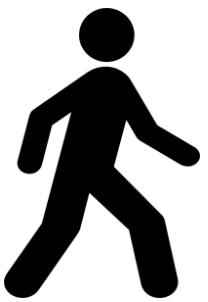
\includegraphics[scale=0.3]{Images/walking_man.png}}
    
    
    % Arrow
    \draw[Green,dashed,->,line width=1mm] (axis cs: 0,5)--(axis cs: 4,5);
    \draw[Green,dashed,->,line width=1mm] (axis cs: 4,5)--(axis cs: 4,0);
    % Walking snow shoe
    \put(8,24){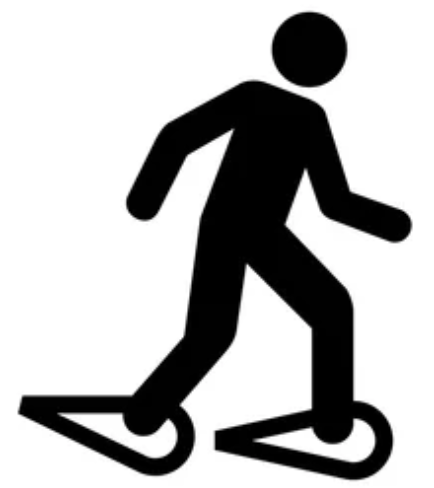
\includegraphics[scale=0.20]{Images/snow_racket_2.png}}
  
    %\addplot [red,line width=0.5mm,no markers, raw gnuplot] gnuplot { plot 'Sand_Sinkage_cm_kPa.dat' smooth sbezier;};
    
    \node[red,right] at (axis cs: 1,75) {\bf Sinkage with normal shoes = 20 cm};
    \node[Green,right] at (axis cs: 1,68) {\bf Sinkage with snow  shoes = 4 cm};
\end{axis}
\end{tikzpicture}
    %\caption{Alger, R. and Osborne, M. (1989)}%Alger, R. and Osborne, M. (1989). Snow characterization field data collection results (Final Report No. ACA90-85-K-002). Keweenaw Research Center, Michigan Technological University, Houghton, MI.}
\end{figure}    

\end{frame}





\begin{frame}{\huge{Thank you!}}
    %For collaborating in this observation lesson.\\
    
    All the materials used in this lesson:
    \begin{itemize}
        \item[*] Slides
        \item[*] Lesson plan
    \end{itemize}
    Can be found online on:\\ % (written in your booklet):\\
    \textbf{GitHub:}\\
    \href{https://github.com/ctriguero/Pressure-Lesson-1-Form2-Methodist-College-Belfast.git}{https://github.com/ctriguero/Pressure-Lesson-1-Form2-Methodist-College-Belfast.git}\\
    and\\
    \textbf{Google Classroom:}\\
\end{frame}



\end{document}